\documentclass[11pt]{article}
\usepackage{times}
\pagestyle{empty}
\parindent 0px
\usepackage{geometry}
 \geometry{
 a4paper,
 total={170mm,257mm},
 left=20mm,
 top=20mm,
 }
 
\title{CS5691: Assignment 3}
\author{Akshat Meena (CS19B052) \\ Shubham Patel (ME19B170)}
\date{}
\usepackage{graphicx}
\graphicspath{ {../../Plots/DTW/Digit}{../../Plots/DTW/Handwritting} }

\begin{document}
\maketitle

\begin{center}
\begin{Large}
A. DTW
\end{Large}
\end{center}

\begin{enumerate}
	\begin{large}
	\item \textbf{Isolated Spoken-Digit}
	\end{large}
	
	\begin{itemize}
		\item From the confusion matrix we see that the accuracy is \textbf{96.7\%} when DTW is applied on the spoken digit data for 20 nearest neighbours.
	\begin{figure}[h]
		\caption{
		\begin{small}
		Confusion matrix for DTW applied on spoken digit data for 20 nearest neighbours
		\end{small}
		}
		\centering
		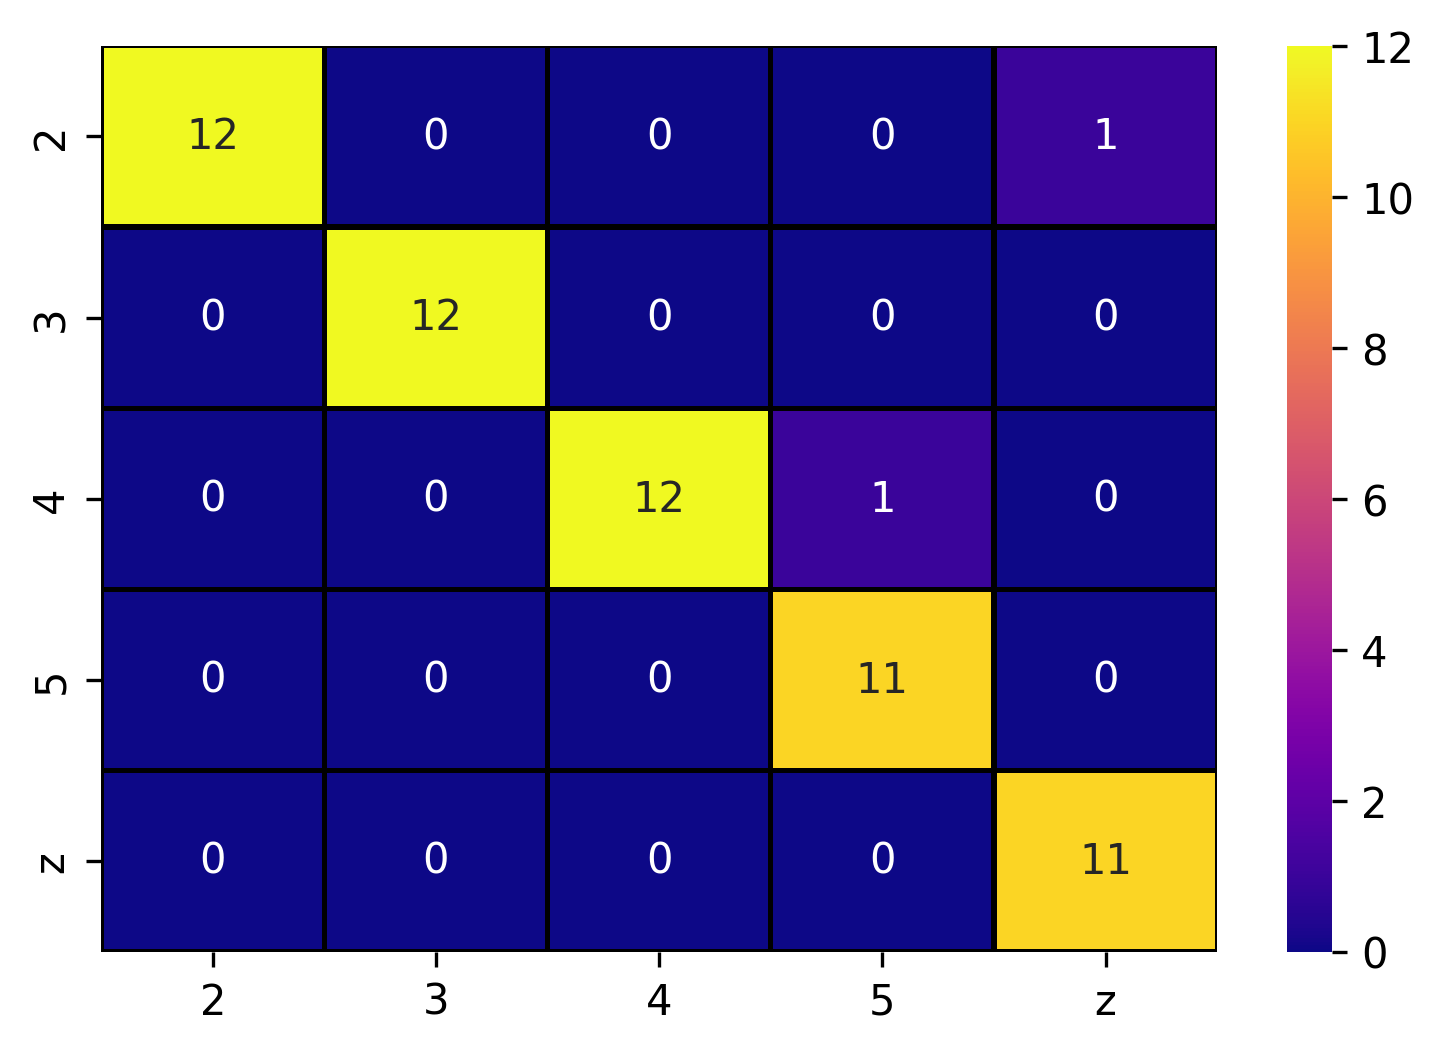
\includegraphics[scale=0.7]{CM_D_20}
	\end{figure}\\
	\item For the 10 nearest neighbours the accuracy increased to \textbf{98.3\%}.
	\begin{figure}[h]
		\caption{
		\begin{small}
		Confusion matrix for DTW applied on spoken digit data for 10 nearest neighbours
		\end{small}
		}
		\centering
		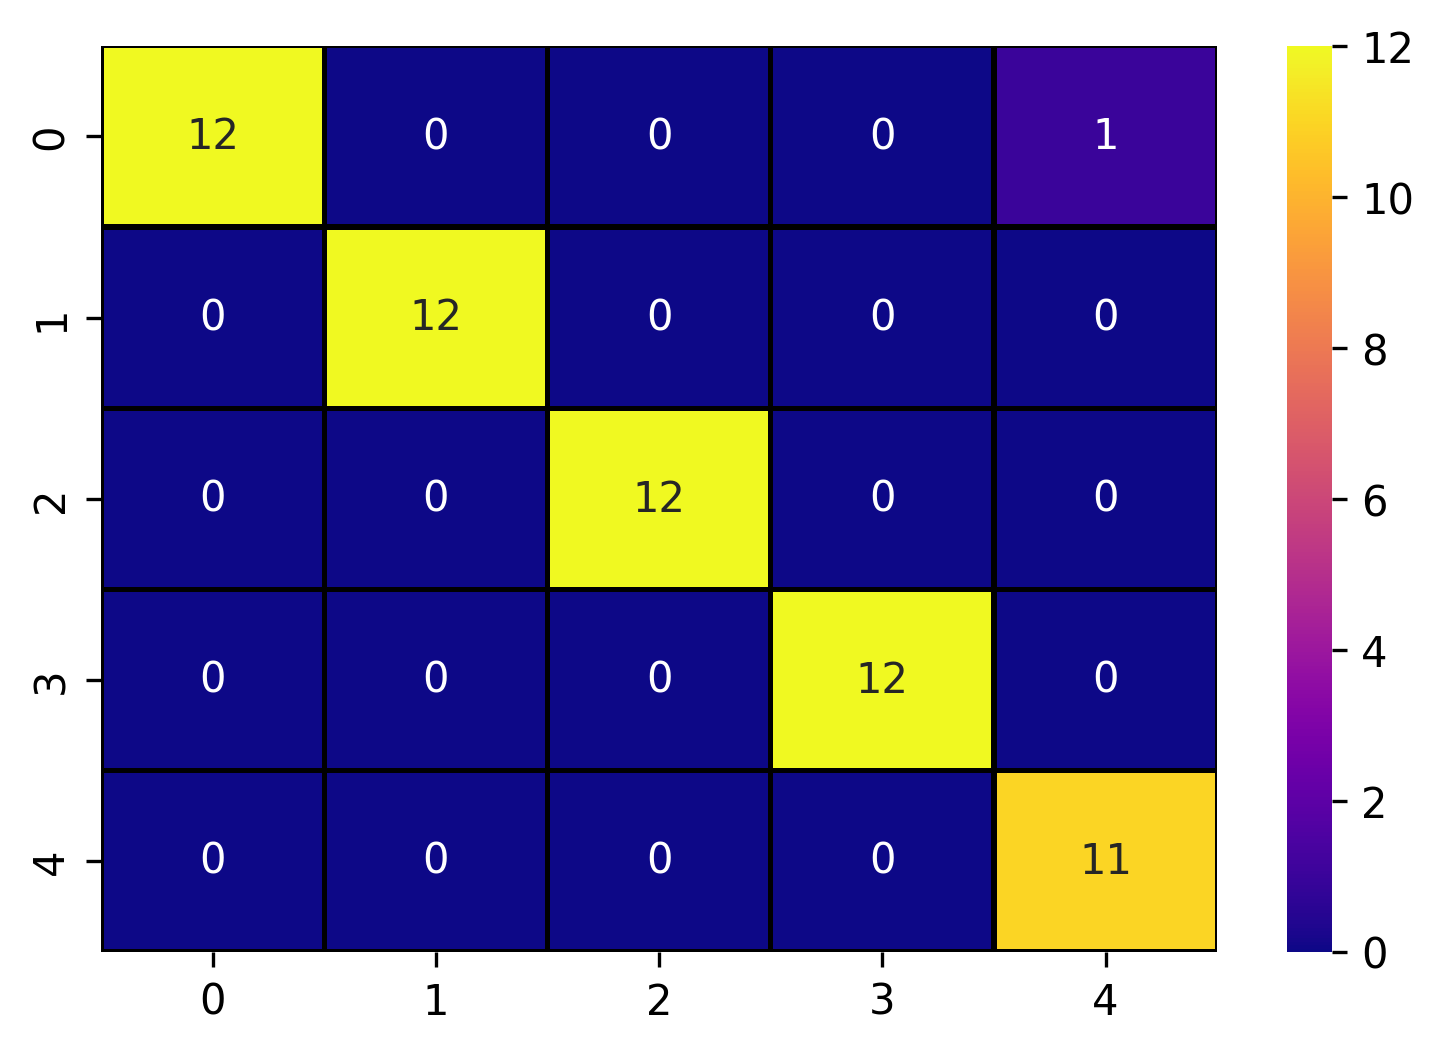
\includegraphics[scale=0.7]{CM_D_10}
	\end{figure}\\
	\item By experimenting with different k-nearest neighbours we observed that the model was having most problem in recognizing the data of 'z' dataset as was confusing it with '2' dataset. And '5' was confused with '4' sometimes.
	\end{itemize}
	
	\begin{large}
	\item \textbf{Online Handwritten-Character}
	\end{large}
	
	\begin{itemize}
		\item When DTW is applied on the handwritten character data for 20 nearest neighbours, we get accuracy of \textbf{60\%}.
		\item we get \textbf{100\%} accuracy for 'dA'. And \textbf{85\%} accuracy for 'a'.
	\begin{figure}[h]
	\caption{
	\begin{small}
	Confusion matrix for DTW applied on handwritten character data for 20 nearest neighbours
	\end{small}
	}
	\centering
	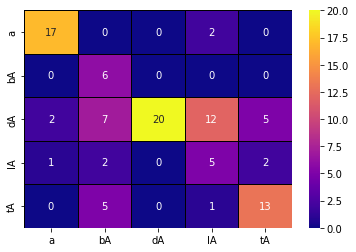
\includegraphics[scale=0.7]{CM_H_20}
	\end{figure}\\
	\item When DTW is applied on the handwritten character data for 60 nearest neighbours, We get accuracy of \textbf{62\%}.
	\item We get better accuracy for 'lA' and 'tA' but lesser for 'bA'.
	\begin{figure}[h]
	\caption{
	\begin{small}
	Confusion matrix for DTW applied on handwritten character data for 60 nearest neighbours
	\end{small}
	}
	\centering
	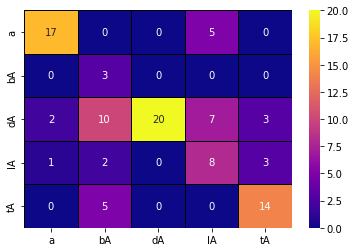
\includegraphics[scale=0.7]{CM_H_60}
	\end{figure}\\
	\item Most of the confusion happens for 'bA' with 'dA' and 'tA'. And 'lA' with 'dA'.
	\item We also observed that when we choose 3 feature vectors (x,y,slope) we were getting lesser accuracy but after using one more feature vector of distance between consecutive points, the accuracy increased slightly.
	\item If we increase the number of significant feature vectors like curvature and other possible then we can get better accuracy.
	\end{itemize}
\end{enumerate}

\end{document}